% Options here are passed to the article class.
% Most common options: 10pt, 11pt, 12pt
\documentclass[10pt]{datasheet}

% Input encoding and typographical rules for English language
\usepackage[utf8]{inputenc}
\usepackage[english]{babel}
\usepackage[english]{isodate}

% tikz is used to draw images in this example, but you can
% also use \includegraphics{}.
\usepackage{graphicx}

% These define global texts that are used in headers and titles.
\title{ES02: Scicraft Hybrid Main Storage}
\author{Jorvp, Obi, CommandLeo, et al.}
\tags{encoded-systems, hybrid-encoded, complete}
\date{25 December 2023}
\revision{Revision 1}
\begin{document}
\maketitle


\section{General Description}
The ES02 Scicraft Hybrid Main Storage is a hybrid encoded storage system, which means it uses regular filters for loose items and encoded box sorting. This system is complete, and is in use in the Scicraft technical Minecraft survival server. \href{https://www.youtube.com/watch?v=8VbCW-Fqjhw}{Youtube video}



% Switch to next column
\vfill\break

\begin{figure}[h]
    \centering
    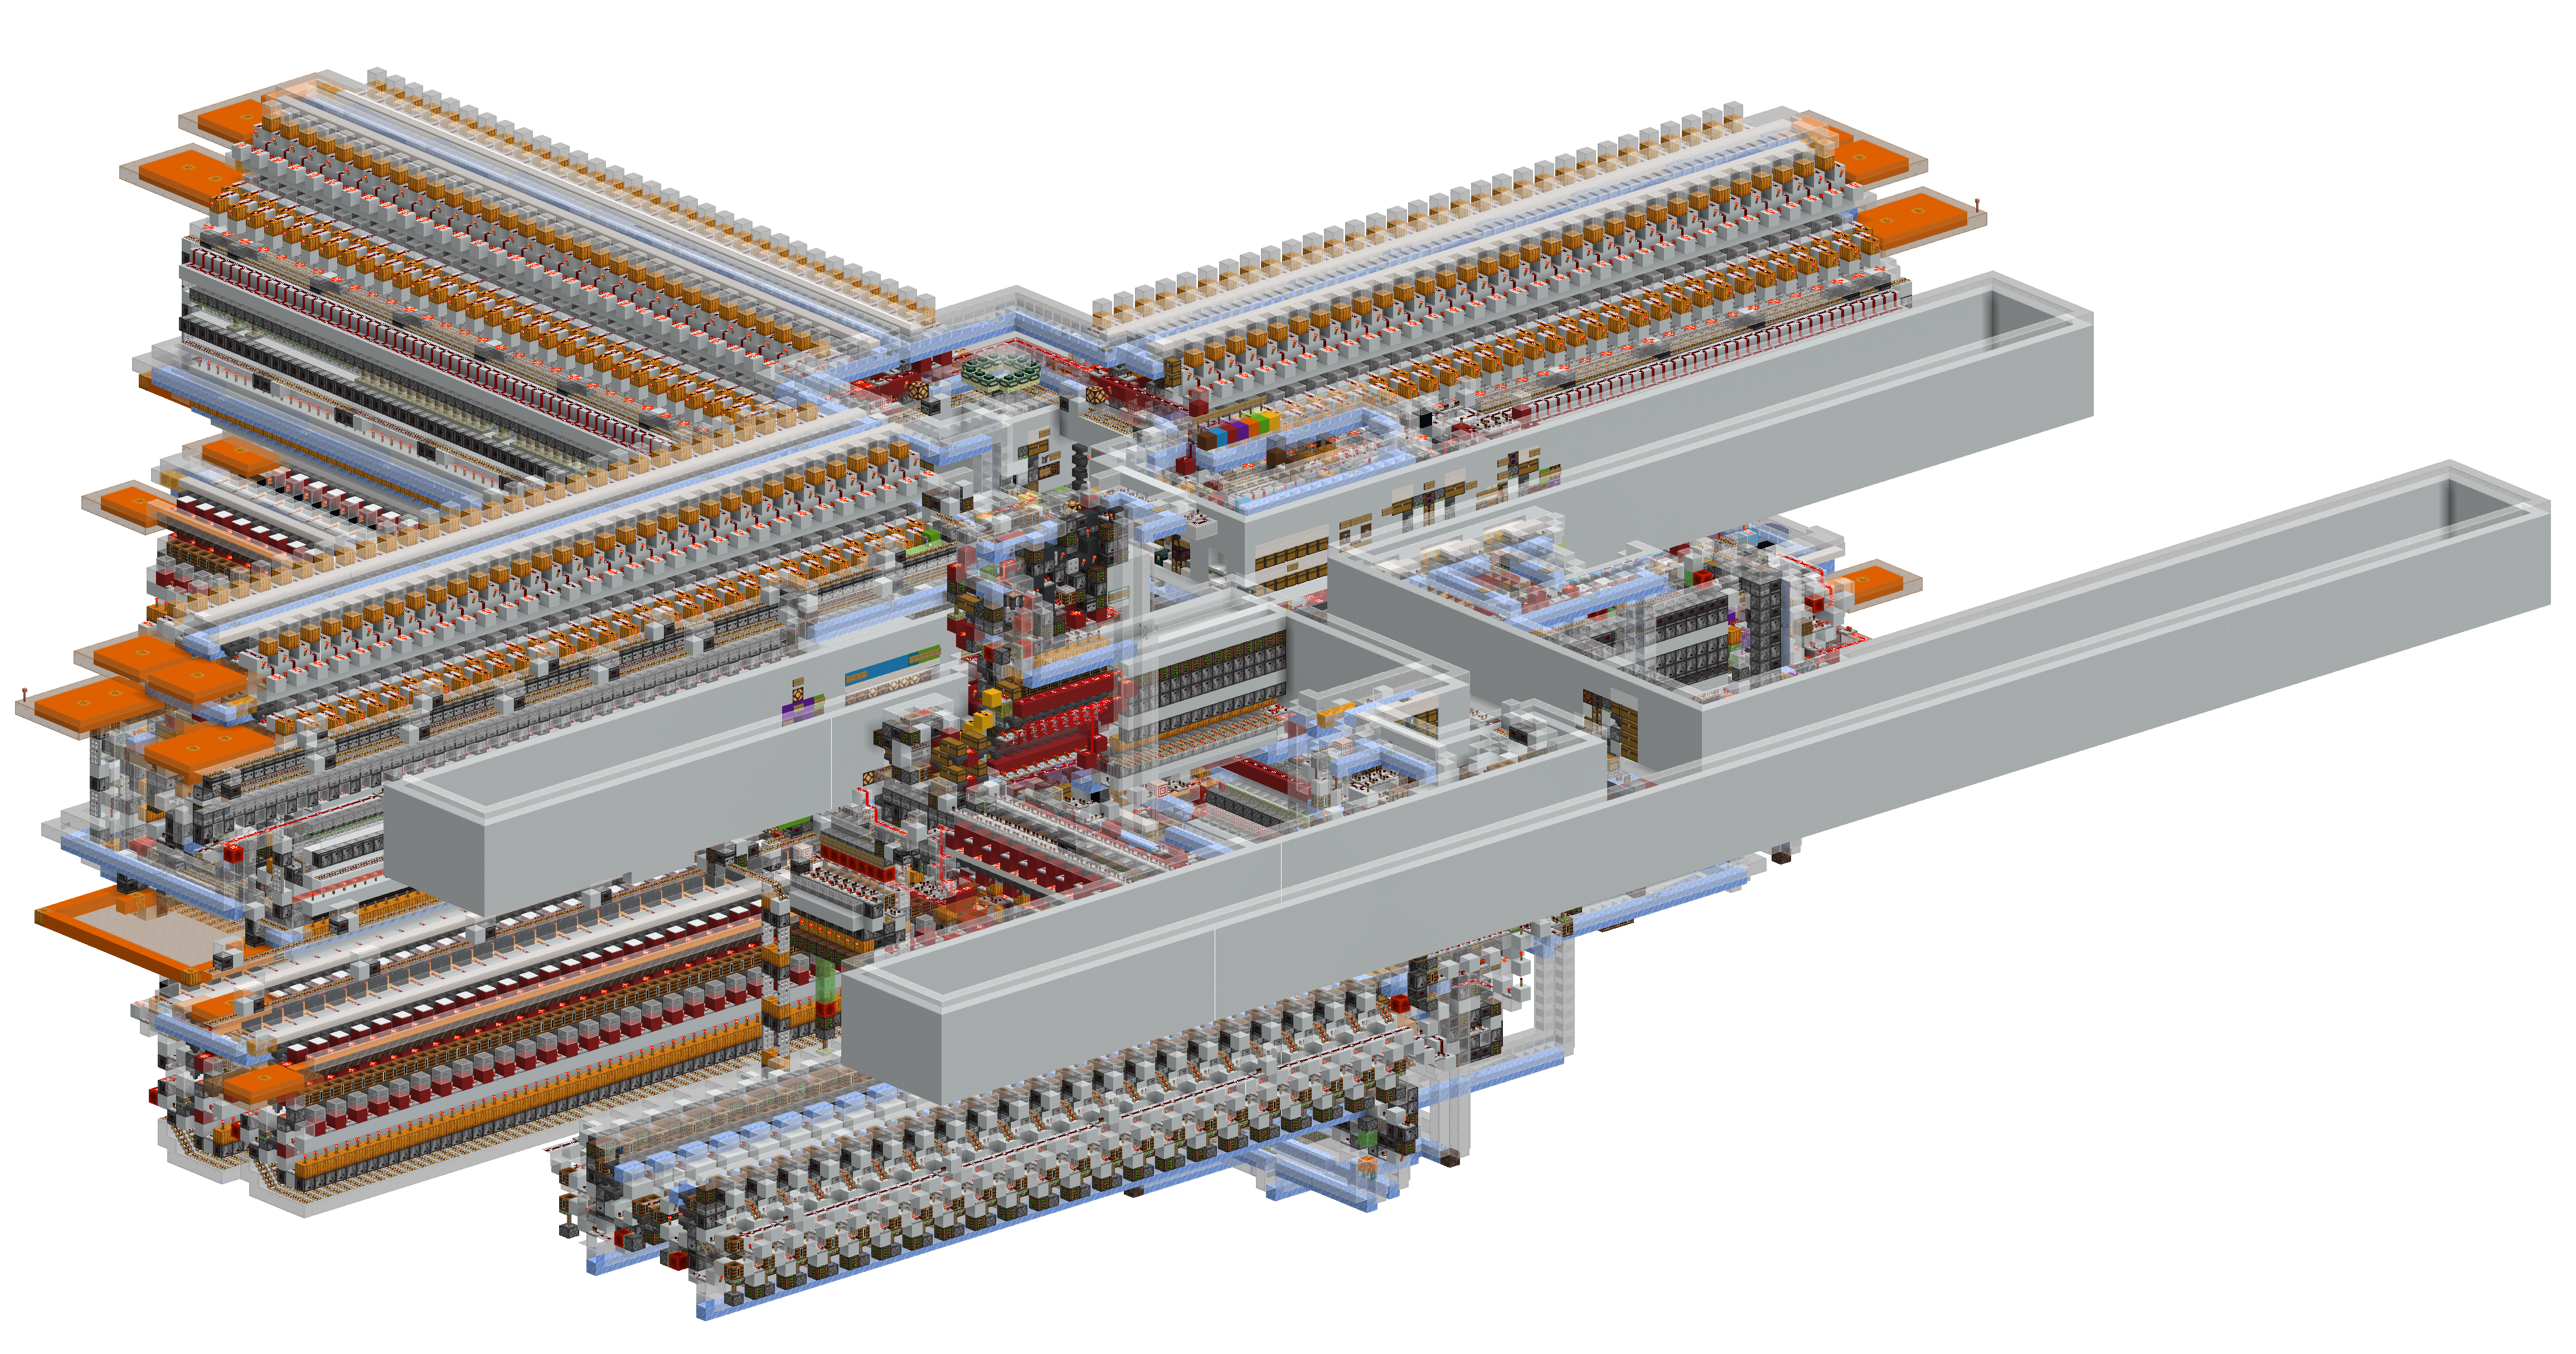
\includegraphics[width=0.45\textwidth]{area_render_1_.png}
    \caption{\centering Scicraft Hybrid Main Storage}
\end{figure}

\begin{figure}[h]
    \centering
    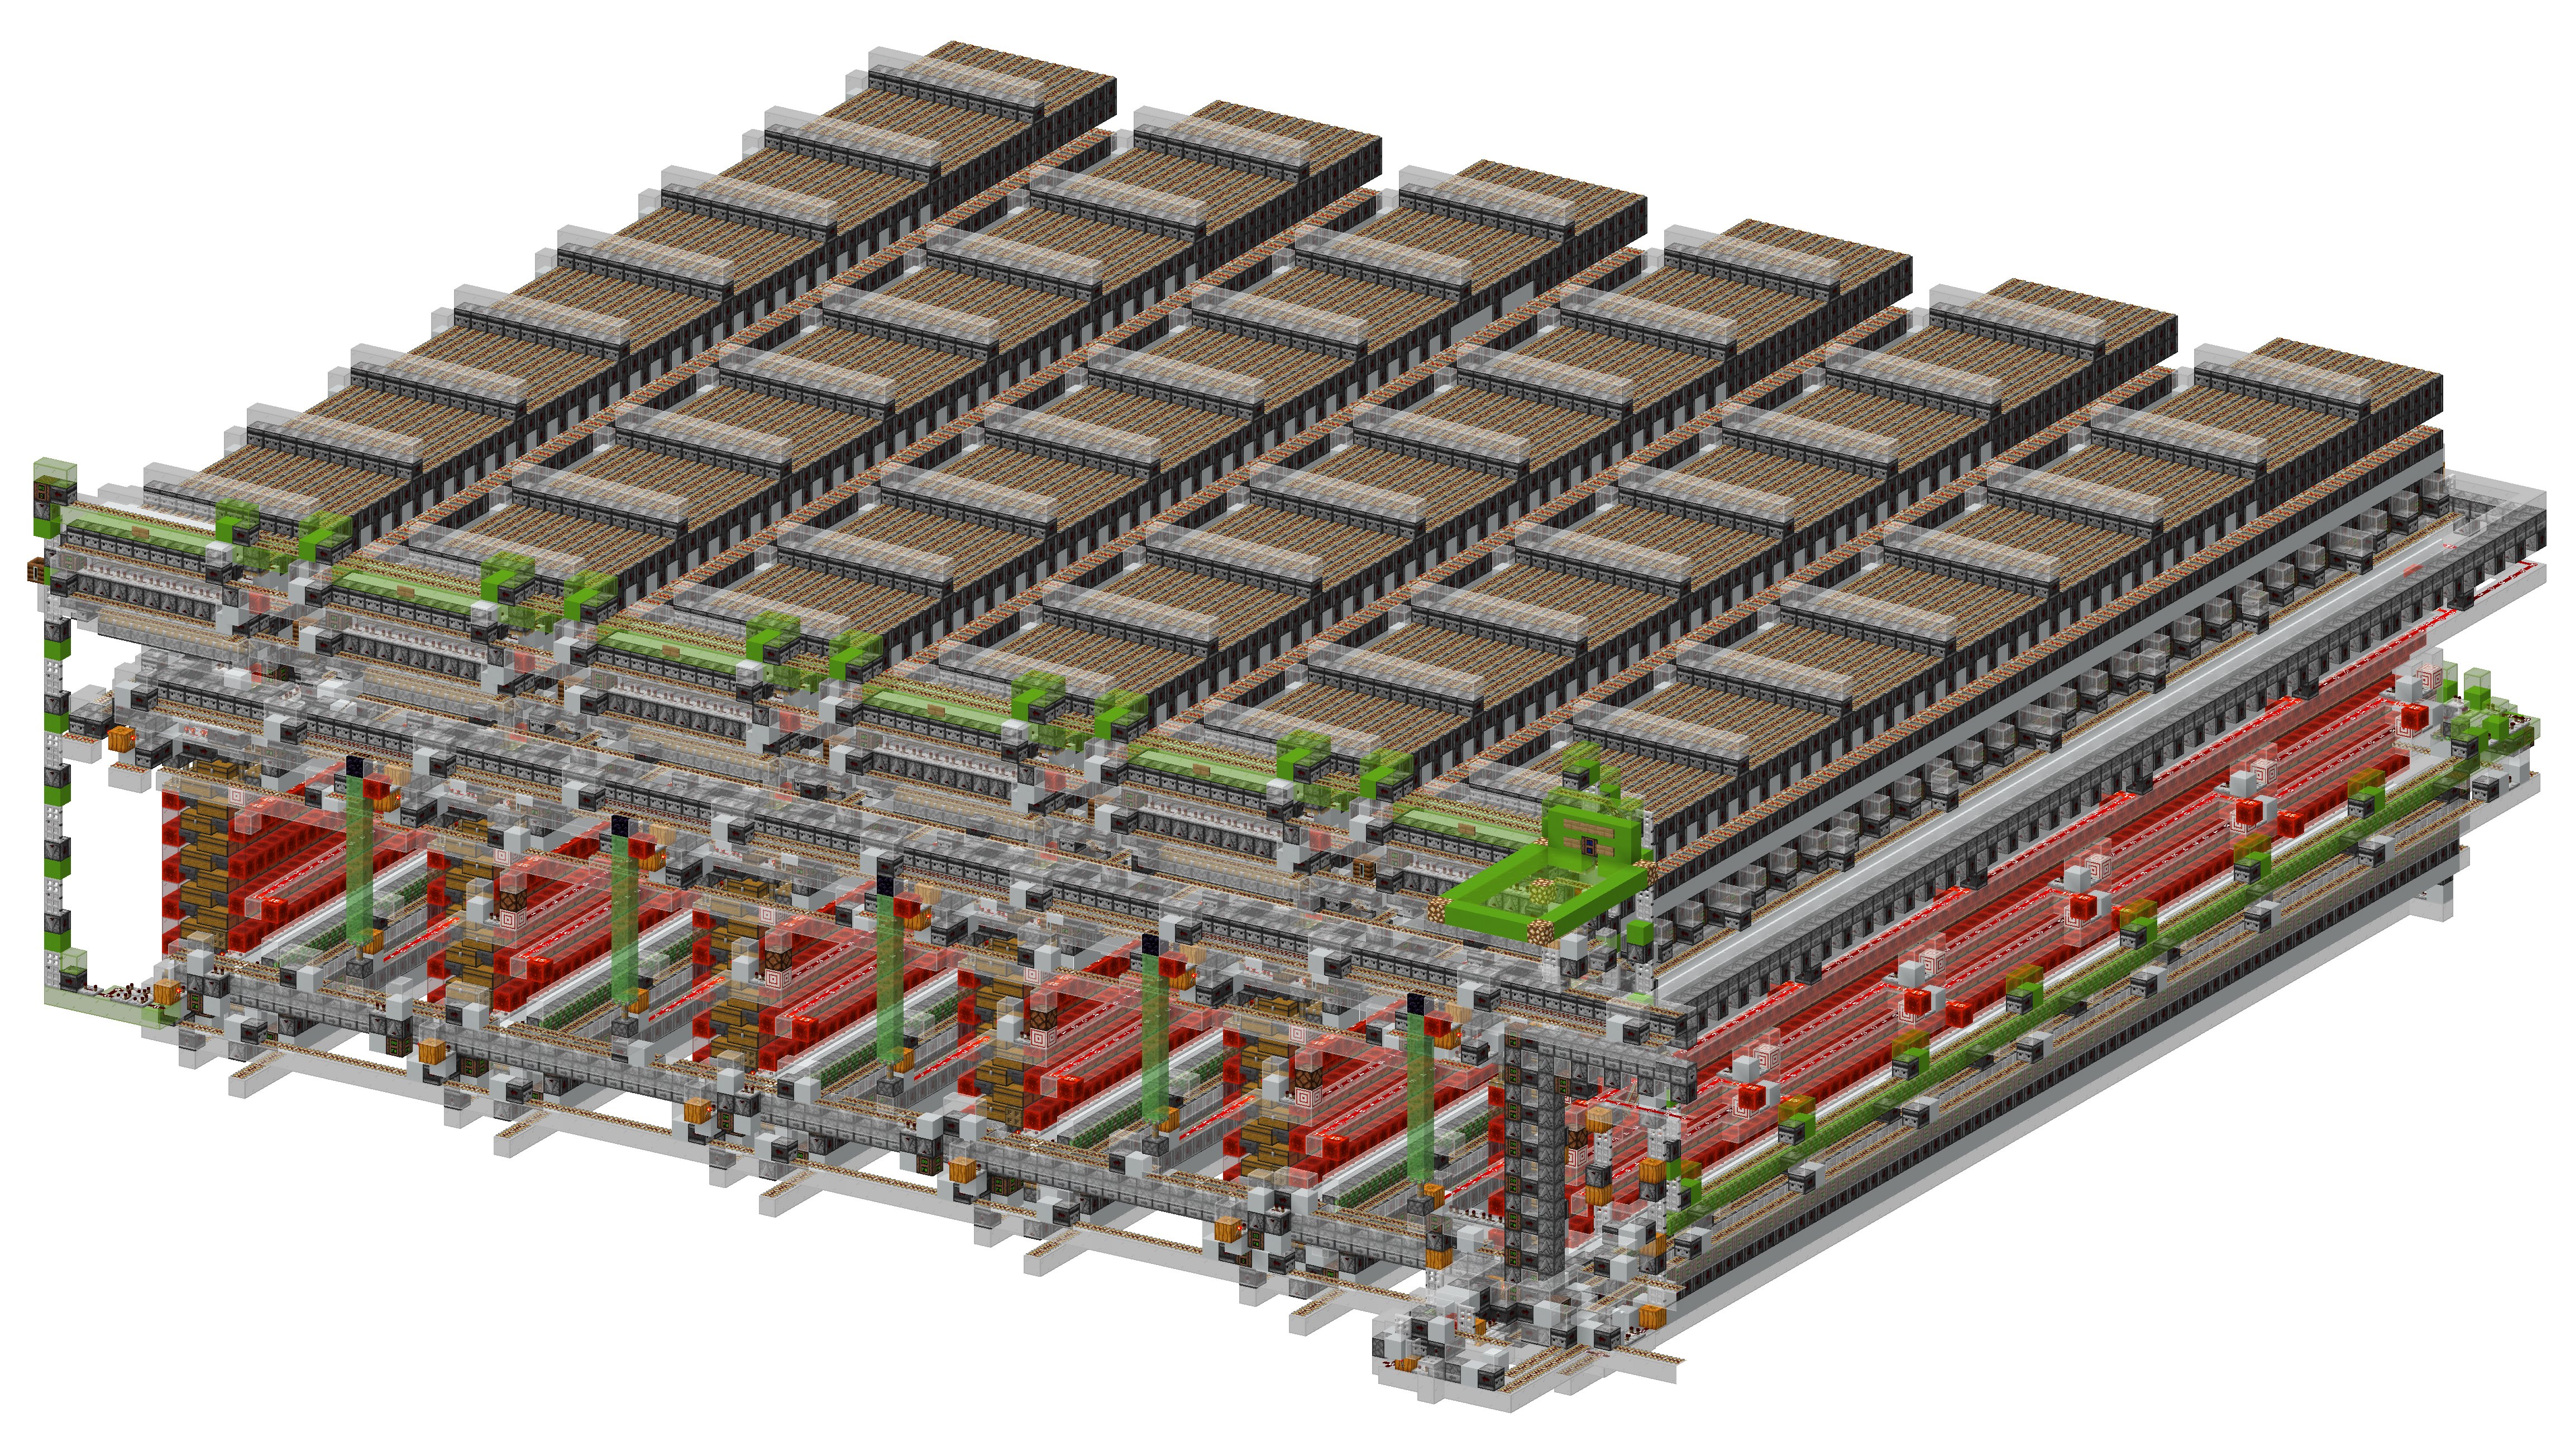
\includegraphics[width=0.45\textwidth]{area_render_2_.png}
    \caption{\centering Remote Bulk}
\end{figure}




\onecolumn

\section{Features}

\begin{itemize}
\item{86.5\% hopper locking. (15\% of the unlocked hoppers are due to the mass crafter. You can get rid of it to achieve almost 99\% hopperlocking.)}
\item{0.5mspt idle, 5mspt active (Ryzen 9 7950X with lithium 1.19.2).}
\item{3 Hybrid Halls, which means both items and boxes in the same hall, which makes for a very interesting item layout.}
\item{Up to 378 Bulk Items, 756 Loose items.}
\item{Fixed item encoded remote bulk.}
\item{CommandLeo's unstackable sorter.}
\item{Parallel unloader, (FITu) which allows for sorting items in parallel.}
\item{Complete item layout with encoder setup.}
\item{Multiple peripherals (furnace array, crafting station, Mass crafter, Box yeeter crafter, etc.)}
\item{Full system status output panel}
\item{Basic error checking, can pause the input if there is a problem}
\item{Not a single Togglestate, which means every latch can be reset, with multiple buttons to reset them if there's a server crash.}
\item{Chunkloaded, bulk chunkloaders only activate when needed.}
\end{itemize}

\section{Applications}

\begin{itemize}
\item{Learning about encoded systems}
\item{Using it as a storage system}
\end{itemize}




% For wide tables, a single column layout is better. It can be switched
% page-by-page.

\section{Device Specifications}

\begin{table}[h]
    \caption{Device Specifications}
    \begin{tabularx}{\textwidth}{l | c c c | c | X}
        \thickhline
        \textbf{Parameter} & \textbf{Min.} & \textbf{Typ.} & \textbf{Max.} &
        \textbf{Unit} & \textbf{Conditions} \\
        MC Version & 1.17 & 1.19.2 & - & MCV & Latest version at time of writing: 1.20.4\\
        \thickhline
\end{tabularx}
\end{table}
\newpage
\section{Testing Data}
\begin{table}[h]
\caption{Executed Tests}
\begin{tabularx}{\textwidth}{l | X}
    \thickhline
    \textbf{Test} & \textbf{Result} \\
    \hline
    SMP test & Tested in production over a year of SMP (Although not very active) without any issues. \\
    \thickhline
\end{tabularx}
\end{table}

\section{Download Information}
\begin{table}[h]
    \caption{Download Information}
    \begin{tabularx}{\textwidth}{l | l | l | X}
        \thickhline
        \textbf{Identifier} & \textbf{MC} & \textbf{File} & \textbf{Description} \\
        \hline
        ES02 & 1.19.2 & \href{https://github.com/Soontech-Annals/Archive/blob/8413f90a054b6c415703bae02badeba7541344f6/Archive/encoded-systems/ES02\%20Scicraft\%20Hybrid\%20Main\%20Storage/ES02\_Scicraft\_Hybrid\_Main\_Storage.zip?raw=1}{ES02\_Scicraft\_Hybrid\_Main\_Storage.zip} & WDL of storage system. \\
        \hline
        \thickhline
    \end{tabularx}
\end{table}

\section{Notes}
\begin{itemize}
\item{Mass Crafter does NOT have chunkloaders. Do not Unload the area while using it! Make sure the subchunk is correct! Masscrafter is locational in that way, due to how mod4 works, it needs to be located in a Y level so the items go through a subchunk}
\end{itemize}

\section{Detailed Credits}
\begin{itemize}
\item{Unstackable Sorter By CommandLeo 1.19}
\item{Encoder by Obi}
\item{Hall by Obi, with tweaks of CommandLeo and some things by jorvp. The original idea was put together by jorvp and FloppyDonkey, the original components are both from Optic.}
\item{Bulk by Obi}
\item{Priority list by Obi}
\item{FIT (First item type unloader) by Glotz, Raffq, Rapscallion and Boyenn}
\item{Mass Crafter by Glotz}
\item{Item Layout by jorvp and Glotz}
\item{Furnace Array by FloppyDonkey}
\item{Crafting stations by CommandLeo}
\end{itemize}

\end{document}

